% Source: tex/chapters/ch06/06_ソフトウェアエンジニアリング運用提供.tex
\subsubsection{ロールバックとデータ移行}

ロールバックとは、新しい版のソフトウェアやデータベースが問題を起こしたとき、正しく動く以前の状態へ戻す活動である。データ移行とは、ソフトウェア変更に合わせてデータ構造や内容を移す活動である。

本番配備前には、ロールバック手順が計画され、練習されるべきである。新しい版が障害や性能劣化を起こした場合、素早く以前の状態へ戻せる必要がある。DevOpsでは、この過程を自動化し、監視結果に応じて自動的に戻すことも可能である。

データ移行がある場合、単にプログラムを戻すだけでは不十分である。データの形式が変わっていると、旧版が新しいデータを読めないことがある。したがって、ロールバック計画には、データをどの状態に戻すか、どこまでの処理を再実行するか、利用者にどの影響があるかを含める必要がある。

\begin{figure}[htbp]
\centering
\IfFileExists{assets/fig-ch06-08.png}{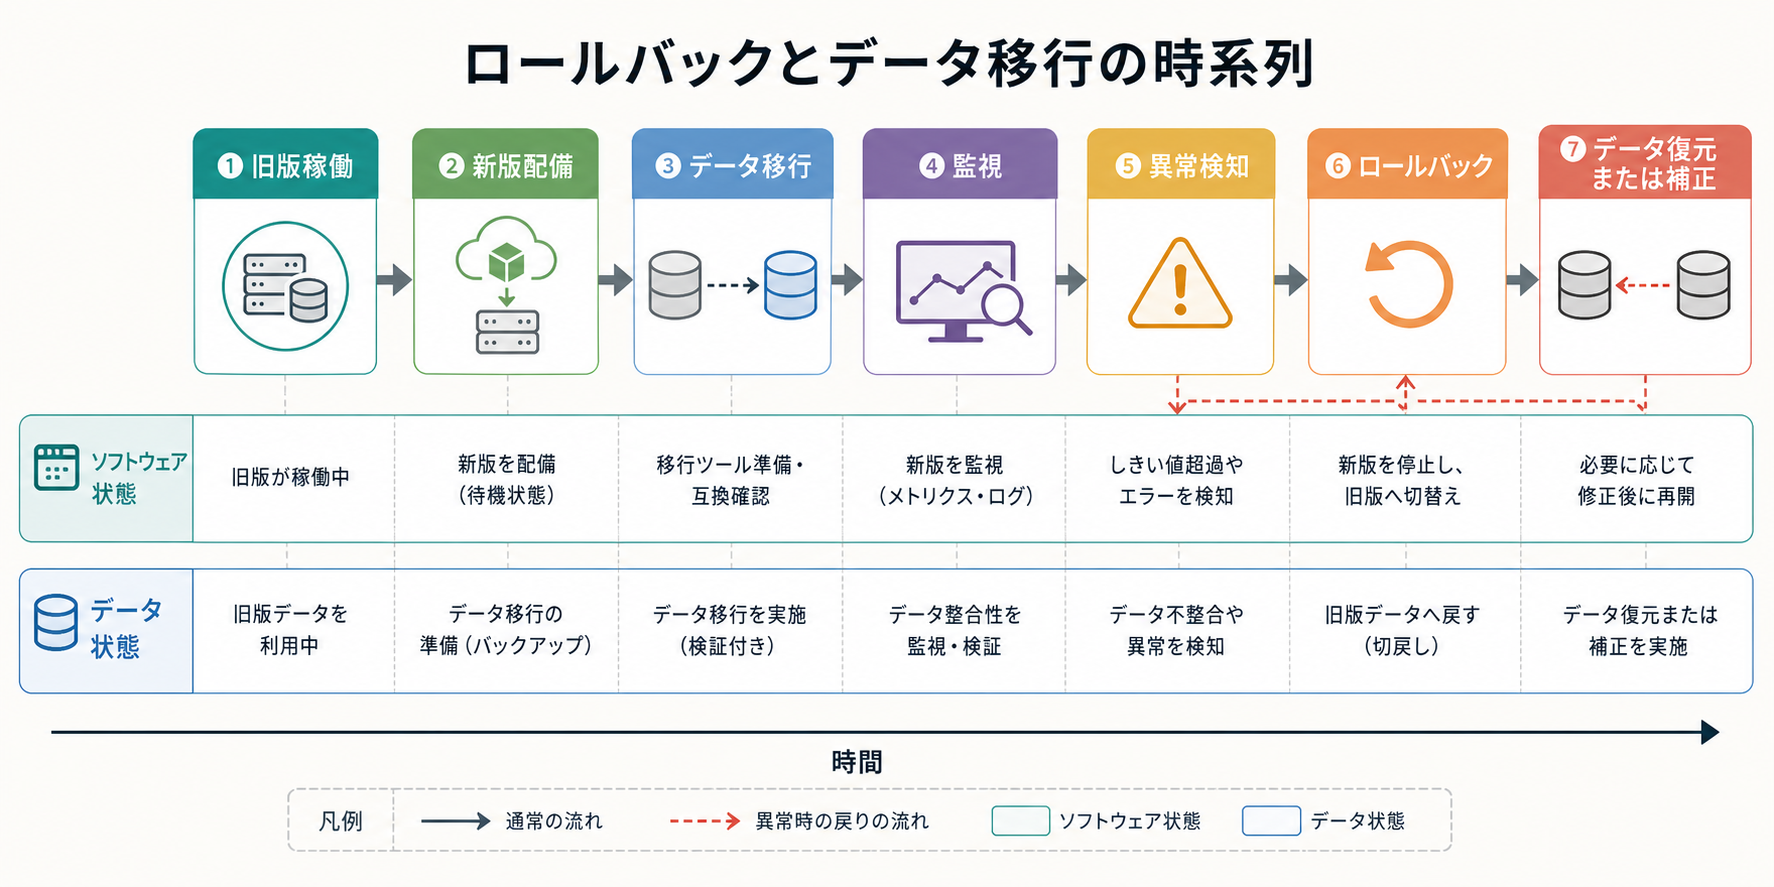
\includegraphics[width=0.96\linewidth]{assets/fig-ch06-08.png}}{\fbox{\parbox[c][48mm][c]{0.9\linewidth}{\centering 画像生成待ち\\ロールバックとデータ移行の時系列}}}
\caption{ロールバックとデータ移行の時系列}
\label{fig:ch06-08}
\end{figure}
